\documentclass{article}
\usepackage{graphicx}
\usepackage{alltt}
\usepackage{amsmath}
\usepackage{amsfonts}
\usepackage{bigstrut}
\usepackage{enumerate}
\usepackage{fancyhdr}
\usepackage[top=.75in, bottom=.95in, left=.75in, right=.75in]{geometry}
\usepackage{float}
\usepackage{lastpage}
\usepackage{tikz}
\usepackage[latin1]{inputenc}
\usepackage{color}
\usepackage{array}
\usepackage{longtable}
\usepackage{calc}
\usepackage{multirow}
\usepackage{hhline}
\usepackage{ifthen}
\usepackage{listings}
\usepackage{circuitikz}
\usepackage{caption}
\definecolor{mygreen}{rgb}{0,0.6,0}
\definecolor{mygray}{rgb}{0.5,0.5,0.5}
\definecolor{mymauve}{rgb}{0.58,0,0.82}
\lstset{ %
  backgroundcolor=\color{white},   % choose the background color; you must add \usepackage{color} or \usepackage{xcolor}; should come as last argument
  basicstyle=\normalsize,        % the size of the fonts that are used for the code
  breakatwhitespace=false,         % sets if automatic breaks should only happen at whitespace
  breaklines=true,                 % sets automatic line breaking
  captionpos=b,                    % sets the caption-position to bottom
  commentstyle=\color{mygreen},    % comment style
  deletekeywords={...},            % if you want to delete keywords from the given language
  escapeinside={\%*}{*)},          % if you want to add LaTeX within your code
  extendedchars=true,              % lets you use non-ASCII characters; for 8-bits encodings only, does not work with UTF-8
  frame=single,	                   % adds a frame around the code
  keepspaces=true,                 % keeps spaces in text, useful for keeping indentation of code (possibly needs columns=flexible)
  keywordstyle=\color{blue},       % keyword style
  language=python,                  % the language of the code
  morekeywords={*,...},            % if you want to add more keywords to the set
  numbers=left,                    % where to put the line-numbers; possible values are (none, left, right)
  numbersep=5pt,                   % how far the line-numbers are from the code
  numberstyle=\tiny\color{mygray}, % the style that is used for the line-numbers
  rulecolor=\color{black},         % if not set, the frame-color may be changed on line-breaks within not-black text (e.g. comments (green here))
  showspaces=false,                % show spaces everywhere adding particular underscores; it overrides 'showstringspaces'
  showstringspaces=false,          % underline spaces within strings only
  showtabs=false,                  % show tabs within strings adding particular underscores
  stepnumber=2,                    % the step between two line-numbers. If it's 1, each line will be numbered
  stringstyle=\color{mymauve},     % string literal style
  tabsize=2,	                   % sets default tabsize to 2 spaces
  title=\lstname                   % show the filename of files included with \lstinputlisting; also try caption instead of title
}
\floatstyle{boxed}
\floatstyle{plain}
\restylefloat{figure}
\pagestyle{fancy}
\fancyhead{}
\fancyfoot{}
\setlength{\headheight}{59.0pt}
\def\inputGnumericTable{}
\fancyhead[CO]{\textbf{Air Force Institute of Technology\\Department of Electrical and Computer Engineering\\
 Computer Communication Networks (CSCE-654) Project \#1\newline \newline Name: Micah Hayden}}
\lhead{\today}
\rhead{Page \thepage{} of \pageref{LastPage} }
\newlength\tindent
\setlength{\tindent}{\parindent}
\setlength{\parindent}{0pt}
\renewcommand{\indent}{\hspace*{\tindent}}
\begin{document}

%\begin{abstract}
%This is my abstract.
%\end{abstract}

\section*{Simulation Setup:}
I utilized the provided FIFO queue sample project as the starting point for my simulation.

\subsection*{Network Configuration}  
My "Tandem Satellite" network consisted of one generator, two FIFO queues/servers, a satellite node, and a sink node.  
The generator, queue, and sink nodes are all the same as given in the FIFO sample (and the same as Project \#1).  
I defined the satellite node as a simple node which handled any incoming message by forwarding it to the following node immediately.  
Due to the distance to the satellite, the simulation needed to account for the propagation delay.
\begin{align*}
& t_{prop} = \frac{d}{c} \hspace{2cm} d = 42,000km  \hspace{1cm} c = 299,792,458 \frac{m}{s} \\
& t_{prop} = \frac{4.2 \times 10^7 m}{299792458 \frac{m}{s}} \\
& \boxed{t_{prop} = 0.1401 ms}
\end{align*}
The satellite node accounted for the propagation delay of communication with the satellite by using a channel delay on the links connecting the satellite to the two queues.
Figure \#\ref{diagram} shows this network setup. 

\begin{figure}[h!]
	\begin{center}
	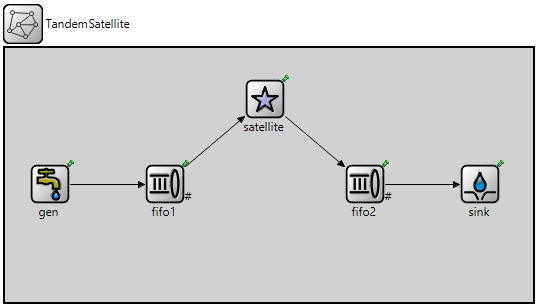
\includegraphics[scale=1.0]{Images/TandemSatellite.PNG}
	\vspace{-.25cm}
	\caption{Network diagram}
	\label{diagram}
	\end{center}
\end{figure}

When a packet arrives at the sink, it generates a packet delay data point as defined in Eq. \#\ref{delay}
\begin{equation}
	\label{delay}
	Packet \, Delay = time_{arrival} - time_{created}
\end{equation}

\newpage
\subsection*{Simulation Time:}  
Before determining a simulation run-time, I calculated $\lambda$, $\mu$, and $\rho$ from the mean service time and interarrival times specified.
Table \#\ref{Parameters} below.
\begin{table}[h!]
\centering
\begin{tabular}{|c|c|c|c|c|} \hline
\textbf{Case \#:} & Interarrival Time (s) & $\mathbf{\lambda}$ & $\mathbf{\mu}$ & $\mathbf{\rho}$ \\ \hline
1 & 1.00 & 1.00 & 2.00 & 0.50 \\ \hline
2 & 0.52 & 1.92 & 2.00 & 0.96 \\ \hline
3 & 0.50 & 2.00 & 2.00 & 1.00 \\ \hline 
\end{tabular}
\caption{Queue Parameters}
\label{Parameters}
\end{table}

Based on these parameters, Case \#3 should become unstable, given a long enough simulation.
I started by running the three cases for 1 hour each.  
However, when I plotted the data, the second case with $t_{IA}=0.52 \, seconds$ actually had a longer average system delay than the final case with $t_{IA}=0.50 \, seconds$, and similar average queue lengths.  
Based on this result, I decided that a longer simulation was needed.  
My final simulation run-time was 10 hours, which generated a result aligning with the expectation given the relationship between $\lambda$ and $\mu$.

\section*{Results \& Analysis:}

\subsection*{System Delay}
Figure \#\ref{DelayPlot} shows the system delay of each queue.

\begin{figure}[h!]
	\begin{center}
	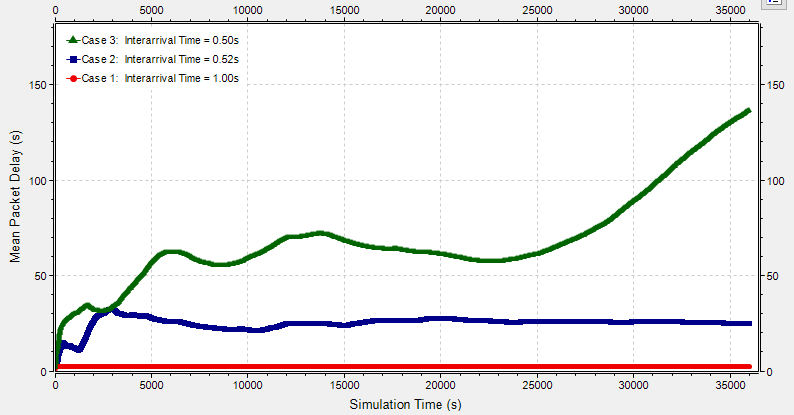
\includegraphics[scale=0.65]{Images/DelayPlot.PNG}
	\vspace{-.25cm}
	\caption{System Delay of varied interarrival times}
	\label{DelayPlot}
	\end{center}
\end{figure}

Case \#1 had an average system delay of 2.02 seconds.  This occurs because $\mu_1 = 2 \cdot \lambda_1$, meaning packets are serviced at twice the arrival rate.
Thus, one would not expect there to be significant delays.
Despite only having a difference of $0.02s$ in interarrival times, the average delay of Cases 2 and 3 were significantly different. Case \#2 had a mean system delay of 26.28 seconds, while the mean delay for Case \#3 was 208.94 seconds.  
This occurs because when $\rho = 1$, the system is unstable and the queue will grow to an infinite length.

\subsection*{Queue Length \& Queue Time}
As shown in Tables 2 \& 3, the average queue lengths and queue times increased relative to the system delay.  
Case \#1 had a low number of packets in the queue because its arrival rate $\lambda_1 = 0.5 \cdot \mu$.

\begin{minipage}{0.5\textwidth}
	\centering
	\begin{tabular}{|c|c|c|c|} \hline
		\textbf{Module} & \textbf{Case \#} & \textbf{Mean (packets)} & \textbf{Std. Dev} \\ \hline
	 fifo1 & 1 & 1.550 & 1.628 \\ \hline
	 fifo1 & 2 & 28.641 & 27.994 \\ \hline
	 fifo1 & 3 & 135.166 & 87.599 \\ \hline
	 fifo2 & 1 & 1.509 & 1.488 \\ \hline
	 fifo2 & 2 & 22.831 & 21.021 \\ \hline
	 fifo2 & 3 & 284.557 & 193.670 \\ \hline
	\end{tabular}
	\captionof{table}{Queue Length }
	\label{qlen}
\end{minipage}  
\begin{minipage}{0.5\textwidth}
	\centering
	\begin{tabular}{|c|c|c|c|} \hline
		\textbf{Module} & \textbf{Case \#} & \textbf{Mean (s)} & \textbf{Std. Dev} \\ \hline
		fifo1 & 1 & 0.517 & 0.912 \\ \hline
		fifo1 & 2 & 14.131 & 14.333 \\ \hline
		fifo1 & 3 & 67.148 & 43.887 \\ \hline
		fifo2 & 1 & 0.504 & 0.862 \\ \hline
		fifo2 & 2 & 11.151 & 10.748 \\ \hline
		fifo2 & 3 & 141.203 & 97.621 \\ \hline
	\end{tabular}
	\captionof{table}{Queue Time}
	\label{qTime}
\end{minipage}

\section*{Conclusions}
This project demonstrated the effects of using deterministic arrival times and service times, which leads to deterministic arrival and service rates.
As long as the service rate is faster than the arrival rate, the system will never queue.

\newpage
\section*{Appendix A:  Figures}

\begin{figure}[h!]
	\begin{center}
	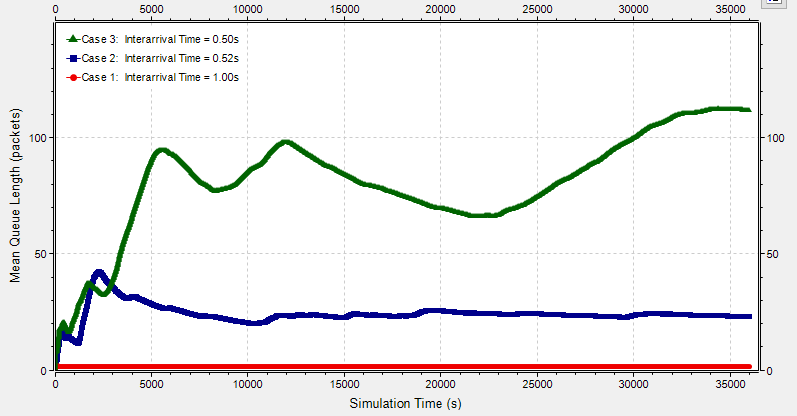
\includegraphics[scale=0.65]{Images/Fifo1_QueueLength.PNG}
	\vspace{-.25cm}
	\caption{Fifo1 Queue Length}
	\label{fifo1_qlen}
	\end{center}
\end{figure}

\begin{figure}[h!]
	\begin{center}
	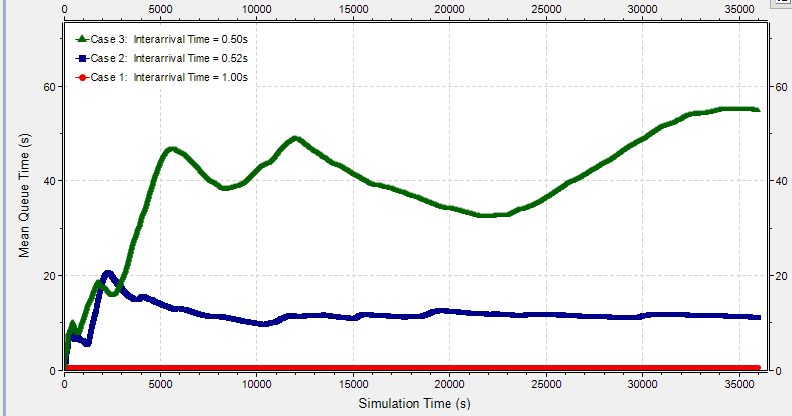
\includegraphics[scale=0.65]{Images/Fifo1_QueueTime.PNG}
	\vspace{-.25cm}
	\caption{Fifo1 Queue Time}
	\label{fifo1_qtime}
	\end{center}
\end{figure}

\begin{figure}[h!]
	\begin{center}
	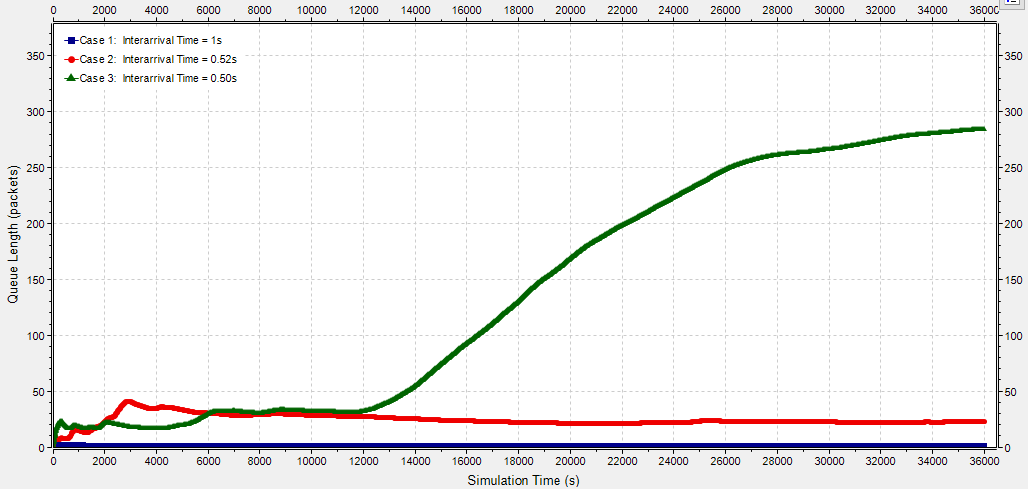
\includegraphics[scale=0.65]{Images/Fifo2_QueueLength.PNG}
	\vspace{-.25cm}
	\caption{Fifo2 Queue Length}
	\label{fifo2_qlen}
	\end{center}
\end{figure}

\begin{figure}[h!]
	\begin{center}
	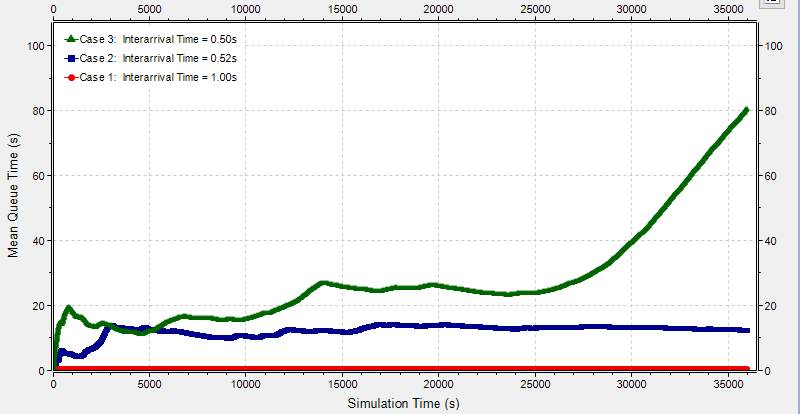
\includegraphics[scale=0.65]{Images/Fifo2_QueueTime.PNG}
	\vspace{-.25cm}
	\caption{Fifo2 Queue Time}
	\label{fifo2_qtime}
	\end{center}
\end{figure}

\end{document}
